%\documentclass[report]{IEEEtran}
\documentclass{article}
\usepackage{footnote}
%\usepackage[font={small}]{caption}
\usepackage{sidecap}
\usepackage{graphicx}
\usepackage{cite}
\usepackage{hyperref}
%\usepackage[stable]{footmisc}
\usepackage{caption}
\usepackage{adjustbox}
\usepackage{subcaption}
\usepackage{algpseudocode}
\usepackage{algorithm}
\usepackage{amsmath}
\usepackage{amssymb}

\begin{document}

\title{Reliable feature point matching}
\author{Jonas Arnfred}

\maketitle

\section{Introduction}
What is the subject of this thesis and in what part lies my 
contribution?
How is the report organized?

\section{Background}
Introduction to Computer Vision
 - Introduce common tasks that we are good at that computers aren't
 - Single in on tasks that we can solve using feature points

Introduction to feature points
 - Global explanation of what they are and how they serve to solve the 
problems mentioned before
 - How do we find them? (Examples making it intuitive why corners are 
nice)
 - How do we describe them? (Relate invariance: Light, Rotation, Noise, 
 Scale, \ldots, Affine)
 - Introduce SIFT and explain how the different problems are tackled in 
SIFT)
 - Talk about other methods and how they are different

Matching feature points
 - What applications require matching?
 - How is matching usually done
 - Segue into related work from paper

\section{Matching feature points}
Basically c/p from paper, but better figures and maybe more explanations
 - Add path about graphs and how they are formed. Make sure to explain 
 the clustering in more detail and make it easier to understand
 - Add a good explanation for new figures and how the precision and 
 recall are calculated. This should appear somewhere before results.
 - Add part on spectral matching and modify accordingly. Make sure to 
 underline how the second plot shows how the geometric method is 
 independent of MMC and that they combined yield greater results.

\subsection{Proposed Matching Methods}
\label{S:MatchingMethods}

\subsubsection{Mirror Match (\emph{MM})}

\begin{figure}
	\centering%
		\begin{subfigure}[t]{\columnwidth}
			\centering
			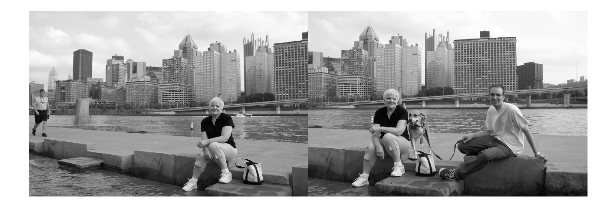
\includegraphics[width=0.85\columnwidth]{images/MMC_pitts_source}
			\caption{Source image pair}
			\label{fig:pitts_source}
		\end{subfigure}%
		\\ %
		\begin{subfigure}[t]{\columnwidth}
			\centering
			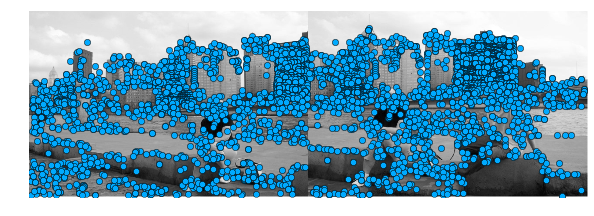
\includegraphics[width=0.85\columnwidth]{images/MMC_pitts_keypoints}
			\caption{Feature points}
			\label{fig:pitts_keypoints}
		\end{subfigure}%
		\\ %add desired spacing between images, e. g. ~, \quad, 
		%\qquad (or a blank line to force the subfigure onto a new line)
		\begin{subfigure}[t]{\columnwidth}
			\centering
			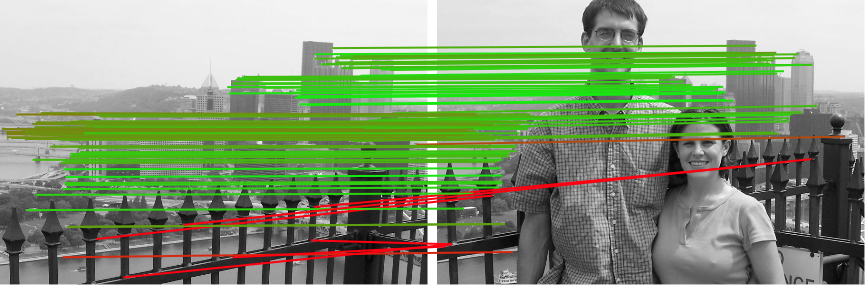
\includegraphics[width=0.85\columnwidth]{images/mirror_match_off}
			\caption{\emph{Ratio}}
			\label{fig:unique}
		\end{subfigure}%
		\\ %add desired spacing between images, e. g. ~, \quad, 
		\begin{subfigure}[t]{\columnwidth}
			\centering
			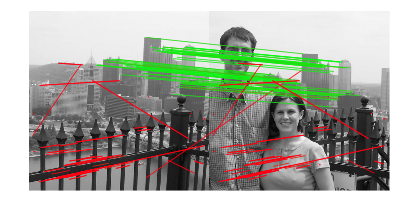
\includegraphics[width=0.85\columnwidth]{images/mirror_match_with_pruned}
			\caption{\emph{MM} intermediate result}
			\label{fig:within}
		\end{subfigure}%
		\\ %add desired spacing between images, e. g. ~, \quad, 
		%\qquad (or a blank line to force the subfigure onto a new line)
		\begin{subfigure}[t]{\columnwidth}
			\centering
			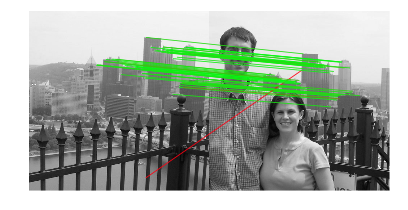
\includegraphics[width=0.85\columnwidth]{images/mirror_match}
			\caption{\emph{MM} final result}
			\label{fig:without}
		\end{subfigure}%
		\\ %add desired spacing between images, e. g. ~, \quad, 
		\begin{subfigure}[t]{\columnwidth}
			\centering
			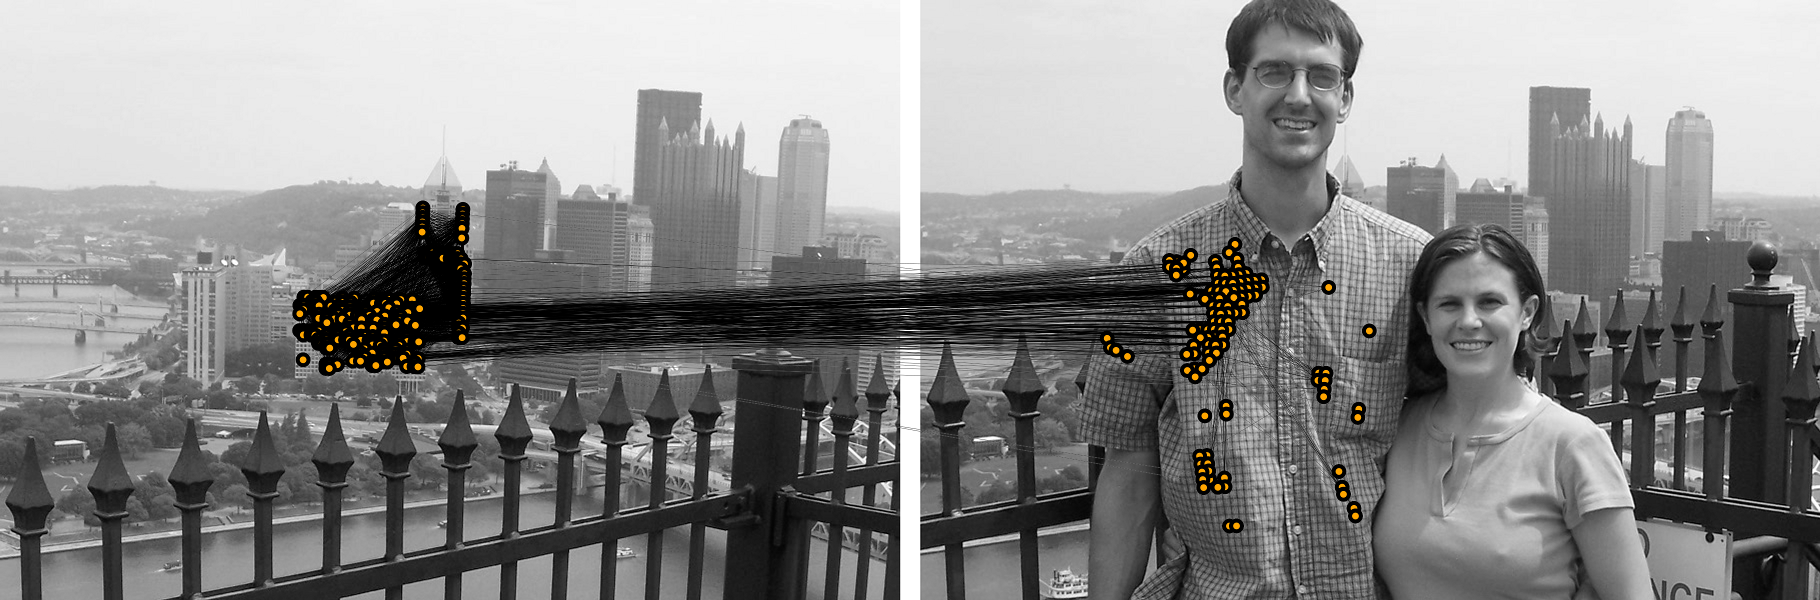
\includegraphics[width=0.85\columnwidth]{images/MMC_partition}
			\caption{\emph{MMC} Partition Example}
			\label{fig:pitts_partition}
		\end{subfigure}%
	\caption{Feature matching with \emph{MM} and \emph{MMC}. Dots represent feature points; green/red lines indicate correct/incorrect matches, respectively; black lines represent edges in the feature graph.  
	(c) Result of \emph{Ratio} matching. 
  (d) All matches found by \emph{MM}, including intra-image matches. 
	(e) Final \emph{MM} result. 
	(f) Example of a partition of feature points after clustering, which 
includes similar feature points from building windows and shirt patterns.}%
	\label{fig:comparemirror}%
\end{figure}%


%
The central idea behind \emph{MM} is to match features of $n$ images by 
taking every feature from all $n$ images and matching it against every 
other feature from the same set. We can then discard the correspondences 
that match two points within the same image. Algorithm~\ref{alg-mm} details  
the implementation of \emph{MM}.
%
\begin{algorithm}
\caption{Mirror Match (\emph{MM})}
\label{alg-mm}
%{\fontsize{10}{10}\selectfont
\begin{algorithmic}
\Require $images$ : set of images, $t \in \mathbb{R}$
\State $matches_{init}\gets \varnothing$
\State $matches_{final}\gets \varnothing$
\State $features\gets \varnothing$
\ForAll{$I_i \in images$} \Comment Acquisition Stage
	\State $features\gets features \cup getFeatures(I_i)$
\EndFor
\ForAll{$f_i \in features$} \Comment Matching Stage
	\State $f_m,f_n \gets get2NNs(f_i, features \setminus 
	\left\{f_i\right\})$
	\State $ratio \gets similarity(f_i, f_n) / similarity(f_i, f_m)$
	\If{$ratio < t$}
		\State $matches_{init} \gets \left(f_i, f_m\right)$
	\EndIf
\EndFor
\ForAll{$\left(f_i, f_j \right) \in matches_{init}$} \Comment Filter 
Stage
\If{$\left(f_j, f_i \right) \in matches_{init} \wedge getImg(f_i) \neq 
getImg(f_j) \wedge \left(f_j, f_i\right) \not\in matches_{final}$}
		\State $matches_{final} \gets (f_i, f_j)$
	\EndIf
\EndFor \\
\Return $matches_{final}$
\end{algorithmic}
%}
\end{algorithm}
%
In the acquisition stage we gather all features in the set of images.  
In the matching stage these features are matched using $k$-nearest 
neighbors.  For any given feature $f_i$ the two most similar neighbors 
are returned, and we calculate the ratio between them as proposed in 
\cite{lowe2004sift}.  Any correspondence with a ratio above the 
threshold supplied will be discarded. Finally in the filter stage we 
check that matches are from different images and discard all matches 
that are not symmetric.
%
%\begin{figure*}
%	\makebox[\textwidth][c]{%
%		\begin{subfigure}[t]{0.32\textwidth}
%			\centering
%			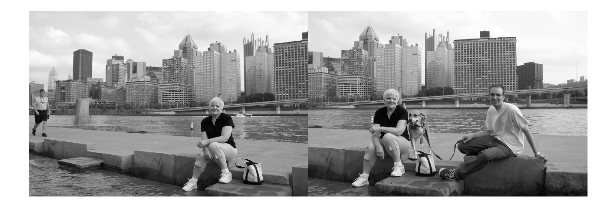
\includegraphics[width=\textwidth]{images/MMC_pitts_source}
%			\caption{Source image pair}
%			\label{fig:pitts_source}
%		\end{subfigure}%
%		\enspace %
%		\begin{subfigure}[t]{0.32\textwidth}
%			\centering
%			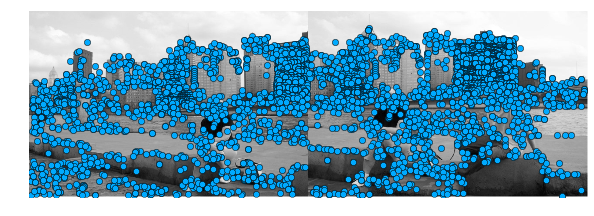
\includegraphics[width=\textwidth]{images/MMC_pitts_keypoints}
%			\caption{Feature points}
%			\label{fig:pitts_keypoints}
%		\end{subfigure}%
%		\enspace %add desired spacing between images, e. g. ~, \quad, 
%		%\qquad (or a blank line to force the subfigure onto a new line)
%		\begin{subfigure}[t]{0.32\textwidth}
%			\centering
%			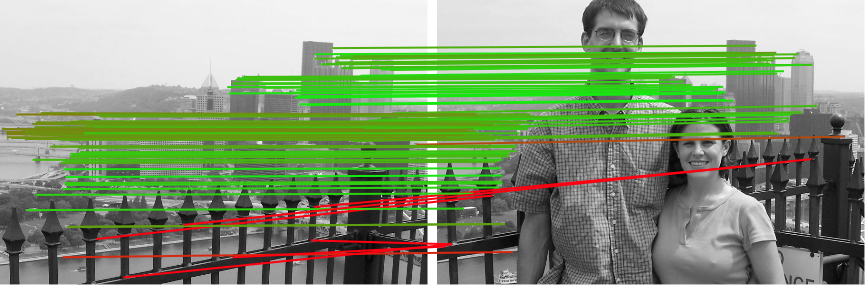
\includegraphics[width=\textwidth]{images/mirror_match_off}
%			\caption{\emph{Ratio}}
%			\label{fig:unique}
%		\end{subfigure}%
%	}
%	\makebox[\textwidth][c]{%
%		\begin{subfigure}[t]{0.32\textwidth}
%			\centering
%			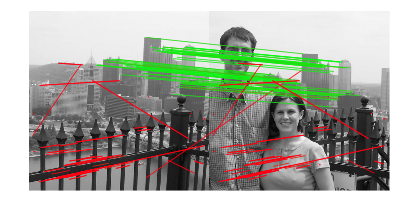
\includegraphics[width=\textwidth]{images/mirror_match_with_pruned}
%			\caption{\emph{MM} intermediate result}
%			\label{fig:within}
%		\end{subfigure}%
%		\enspace %add desired spacing between images, e. g. ~, \quad, 
%		%\qquad (or a blank line to force the subfigure onto a new line)
%		\begin{subfigure}[t]{0.32\textwidth}
%			\centering
%			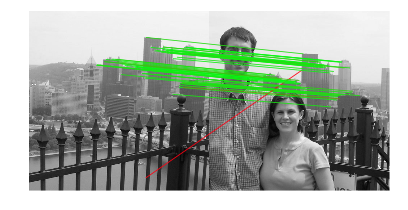
\includegraphics[width=\textwidth]{images/mirror_match}
%			\caption{\emph{MM} final result}
%			\label{fig:without}
%		\end{subfigure}%
%		\enspace%
%		\begin{subfigure}[t]{0.32\textwidth}
%			\centering
%			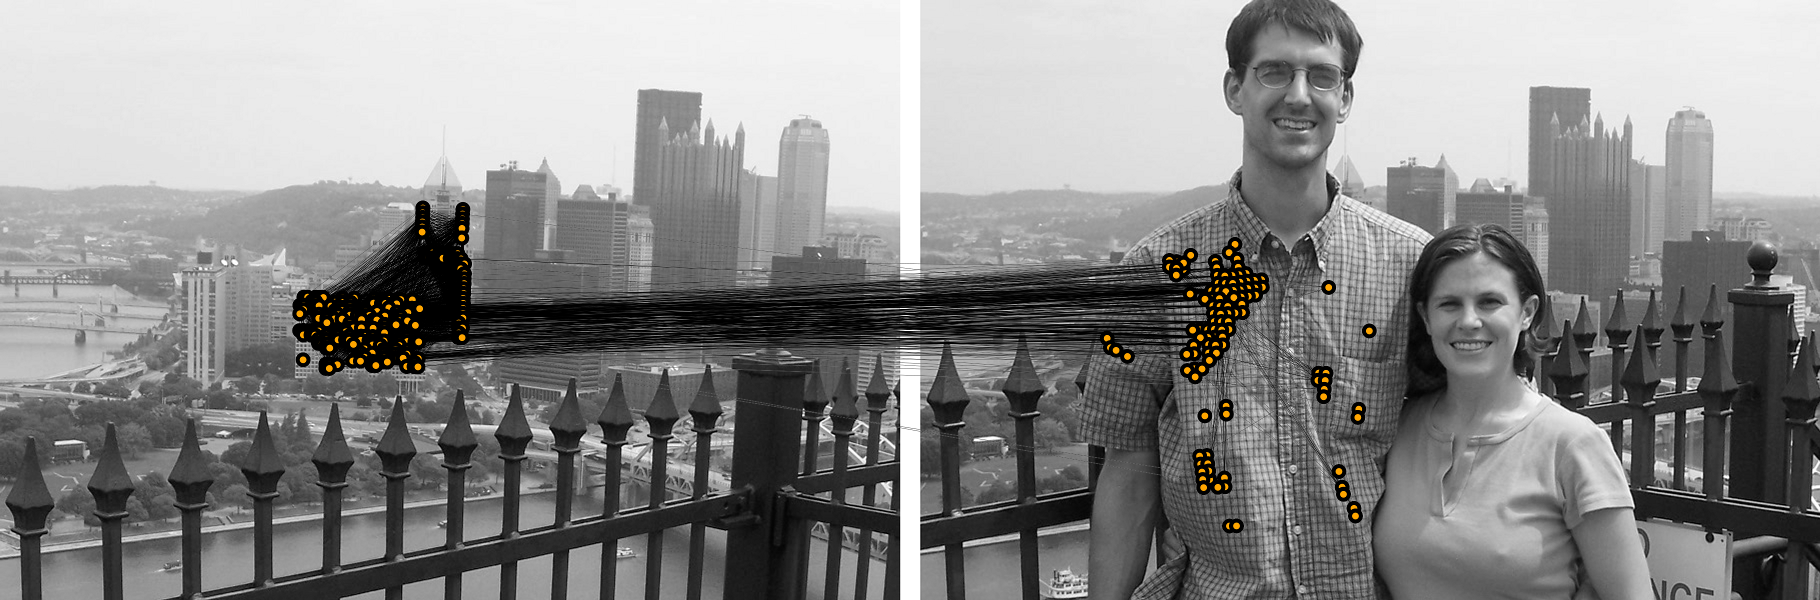
\includegraphics[width=\textwidth]{images/MMC_partition}
%			\caption{\emph{MMC} Partition Example}
%			\label{fig:pitts_partition}
%		\end{subfigure}%
%	}%
%	\caption{Illustration of feature matching with \emph{MM} and \emph{MMC}. Dots represent feature points; green/red lines indicate %correct/incorrect matches, respectively; black lines represent edges in the feature graph.  
%(c) Result of \emph{Ratio} matching the two images.% 
%  (d) All matches found by \emph{MM}, including matches between points in the same image. 
%	(e) Final \emph{MM} result with the intra-image matches removed. 
%	(f) Example of a partition of feature points after clustering. This partition 
%includes similar feature points around the windows of a building and the patterns of a shirt.}%
%	\label{fig:comparemirror}%
%\end{figure*}%


Figure~\ref{fig:comparemirror} illustrates the benefits of \emph{MM} 
using an example image pair from the Gallagher dataset 
\cite{gallagher2008}.
With \emph{Ratio} (Figure~\ref{fig:unique}), many incorrect matches occur 
in the fence towards the bottom of the image.
When we match all feature points together, many of these incorrect 
matches are eliminated, because points in the fence match with other 
points in the fence in the same image (Figures~\ref{fig:within} and
\ref{fig:without}).


\subsubsection{Mirror Match with Clustering (\emph{MMC})}
%
In contrast to \emph{MM}, \emph{MMC} diverges from traditional 
non-geometric feature matching by clustering feature points by 
similarity. This process yields partitions of fairly similar feature 
points that we can match using the same approach as \emph{MM}.  
Algorithm~\ref{alg-mmc} shows the pseudocode implementation of \emph{MMC}.

Before we introduce the implementation details we will go over the 
problem of graph clustering and how it relates to feature matching.

Given a set of feature points from two images, $im_1$ and $im_2$: $F_k = 
\{k_i, k_j$ for $k_i \in im_1, k_j \in im_2\}$ as well as a matching 
function $M(k_i, k_j) \rightarrow \mathbb{R}$ that takes two feature 
points in an image and returns their matching score, we can define a 
matrix $A$ where each element $A_ij = M(k_i, k_j)$. A can be interpreted 
as the \emph{adjecency matrix} of the fully connected graph where each 
vertex corresponds to a keypoint and the edge between two vertices has a 
weight equal to the distance between the two corresponding keypoints.

This representation reduces the problem of partitioning the keypoints 
into groups to that of graph clustering or community structure depending 
on the context. In the literature there are various ways of clustering a 
graph according to different measures of what constitutes an optimal 
partitioning. Traditionally the most used clustering algorithms have 
been K-means and spectral clustering, but in recent years a host of new 
algorithms have been proposed based on both Newman's concept of graph 
modularity\footnote{Introduced in \cite{girvan2002}, discussed in 
\cite{brandes2007} and used in \cite{blondel2008} as well as others} as 
well as information theoretical measures\footnote{See for example 
\cite{rosvall2008}} and the Potts spin model from physics\footnote{Used 
in \cite{ronhovde2009}} just to mention a few approaches. Many of the 
new algorithms differ from K-means clustering and Spectral clustering 
in that they do not require the number of expected to clusters to be 
specified beforehand\footnote{Among the aforementioned methods, this is 
true for \cite{blondel2008} and \cite{rosvall2008}}.  Furthermore, on 
tests done using randomly generated graphs with a known partitioning 
\cite{blondel2008}, \cite{rosvall2008} and \cite{ronhovde2009} perform 
markedly better than spectral clustering and 
K-means\cite{lancichinetti2009}.

The performance of clustering algorithms is a complicated issue, since 
an optimal clustering given the same graph can vary depending on the 
application. Spectral clustering for example will usually return a 
partitioning where each partition is roughly equal in size\footnote{As 
mentioned in \cite{von2007}} while the Louvain 
clustering\cite{blondel2008} might return partitions of very uneven 
size, even if the modularity measurement has been shown to penalize very 
small clusters\cite{brandes2007}. Both behaviours can be beneficial 
depending on the application, but when clustering feature points, 
maintaining clusters of an even size usually means that some clusters 
will be '\emph{catch-all}' clusters where the feature points that do 
not fit anywhere else are grouped together. The necessity of specifying 
the amount of partitions in for example Spectral clustering or Pott's 
model clustering further exacerbates the issue since smaller partitions 
are then combined into one to achieve the right amount of partitions.

%
\begin{algorithm}
\caption{Mirror Match with Clustering (\emph{MMC})}
\label{alg-mmc}
%{\fontsize{10}{10}\selectfont
\begin{algorithmic}
\Require $images$ : set of images, $t \in \mathbb{R}$
\State $M\gets \varnothing$
\State $F\gets \varnothing$
\ForAll{$I_i \in images$} \Comment Gather features
	\State $f_i\gets getFeatures(I_i)$
	\State $F\gets F \cup f_i$
\EndFor
\State $A\gets getAdjacencyMatrix(f_1, f_2,\; \ldots \;, f_n)$
\State $A_{norm}\gets 1 - normalize(A)$
\State $A_{pruned}\gets pruneEdges(A_{norm},\alpha)$
\State $P\gets cluster(A_{pruned})$
\ForAll{$p \in P$} \Comment p is a set of feature points
	\State $M\gets M \cup getMatches(p, t, F)$
\EndFor \\
\Return matches
\end{algorithmic}
%}
\end{algorithm}

\begin{figure}[t]
    \centering
\makebox[\textwidth][c]{%
    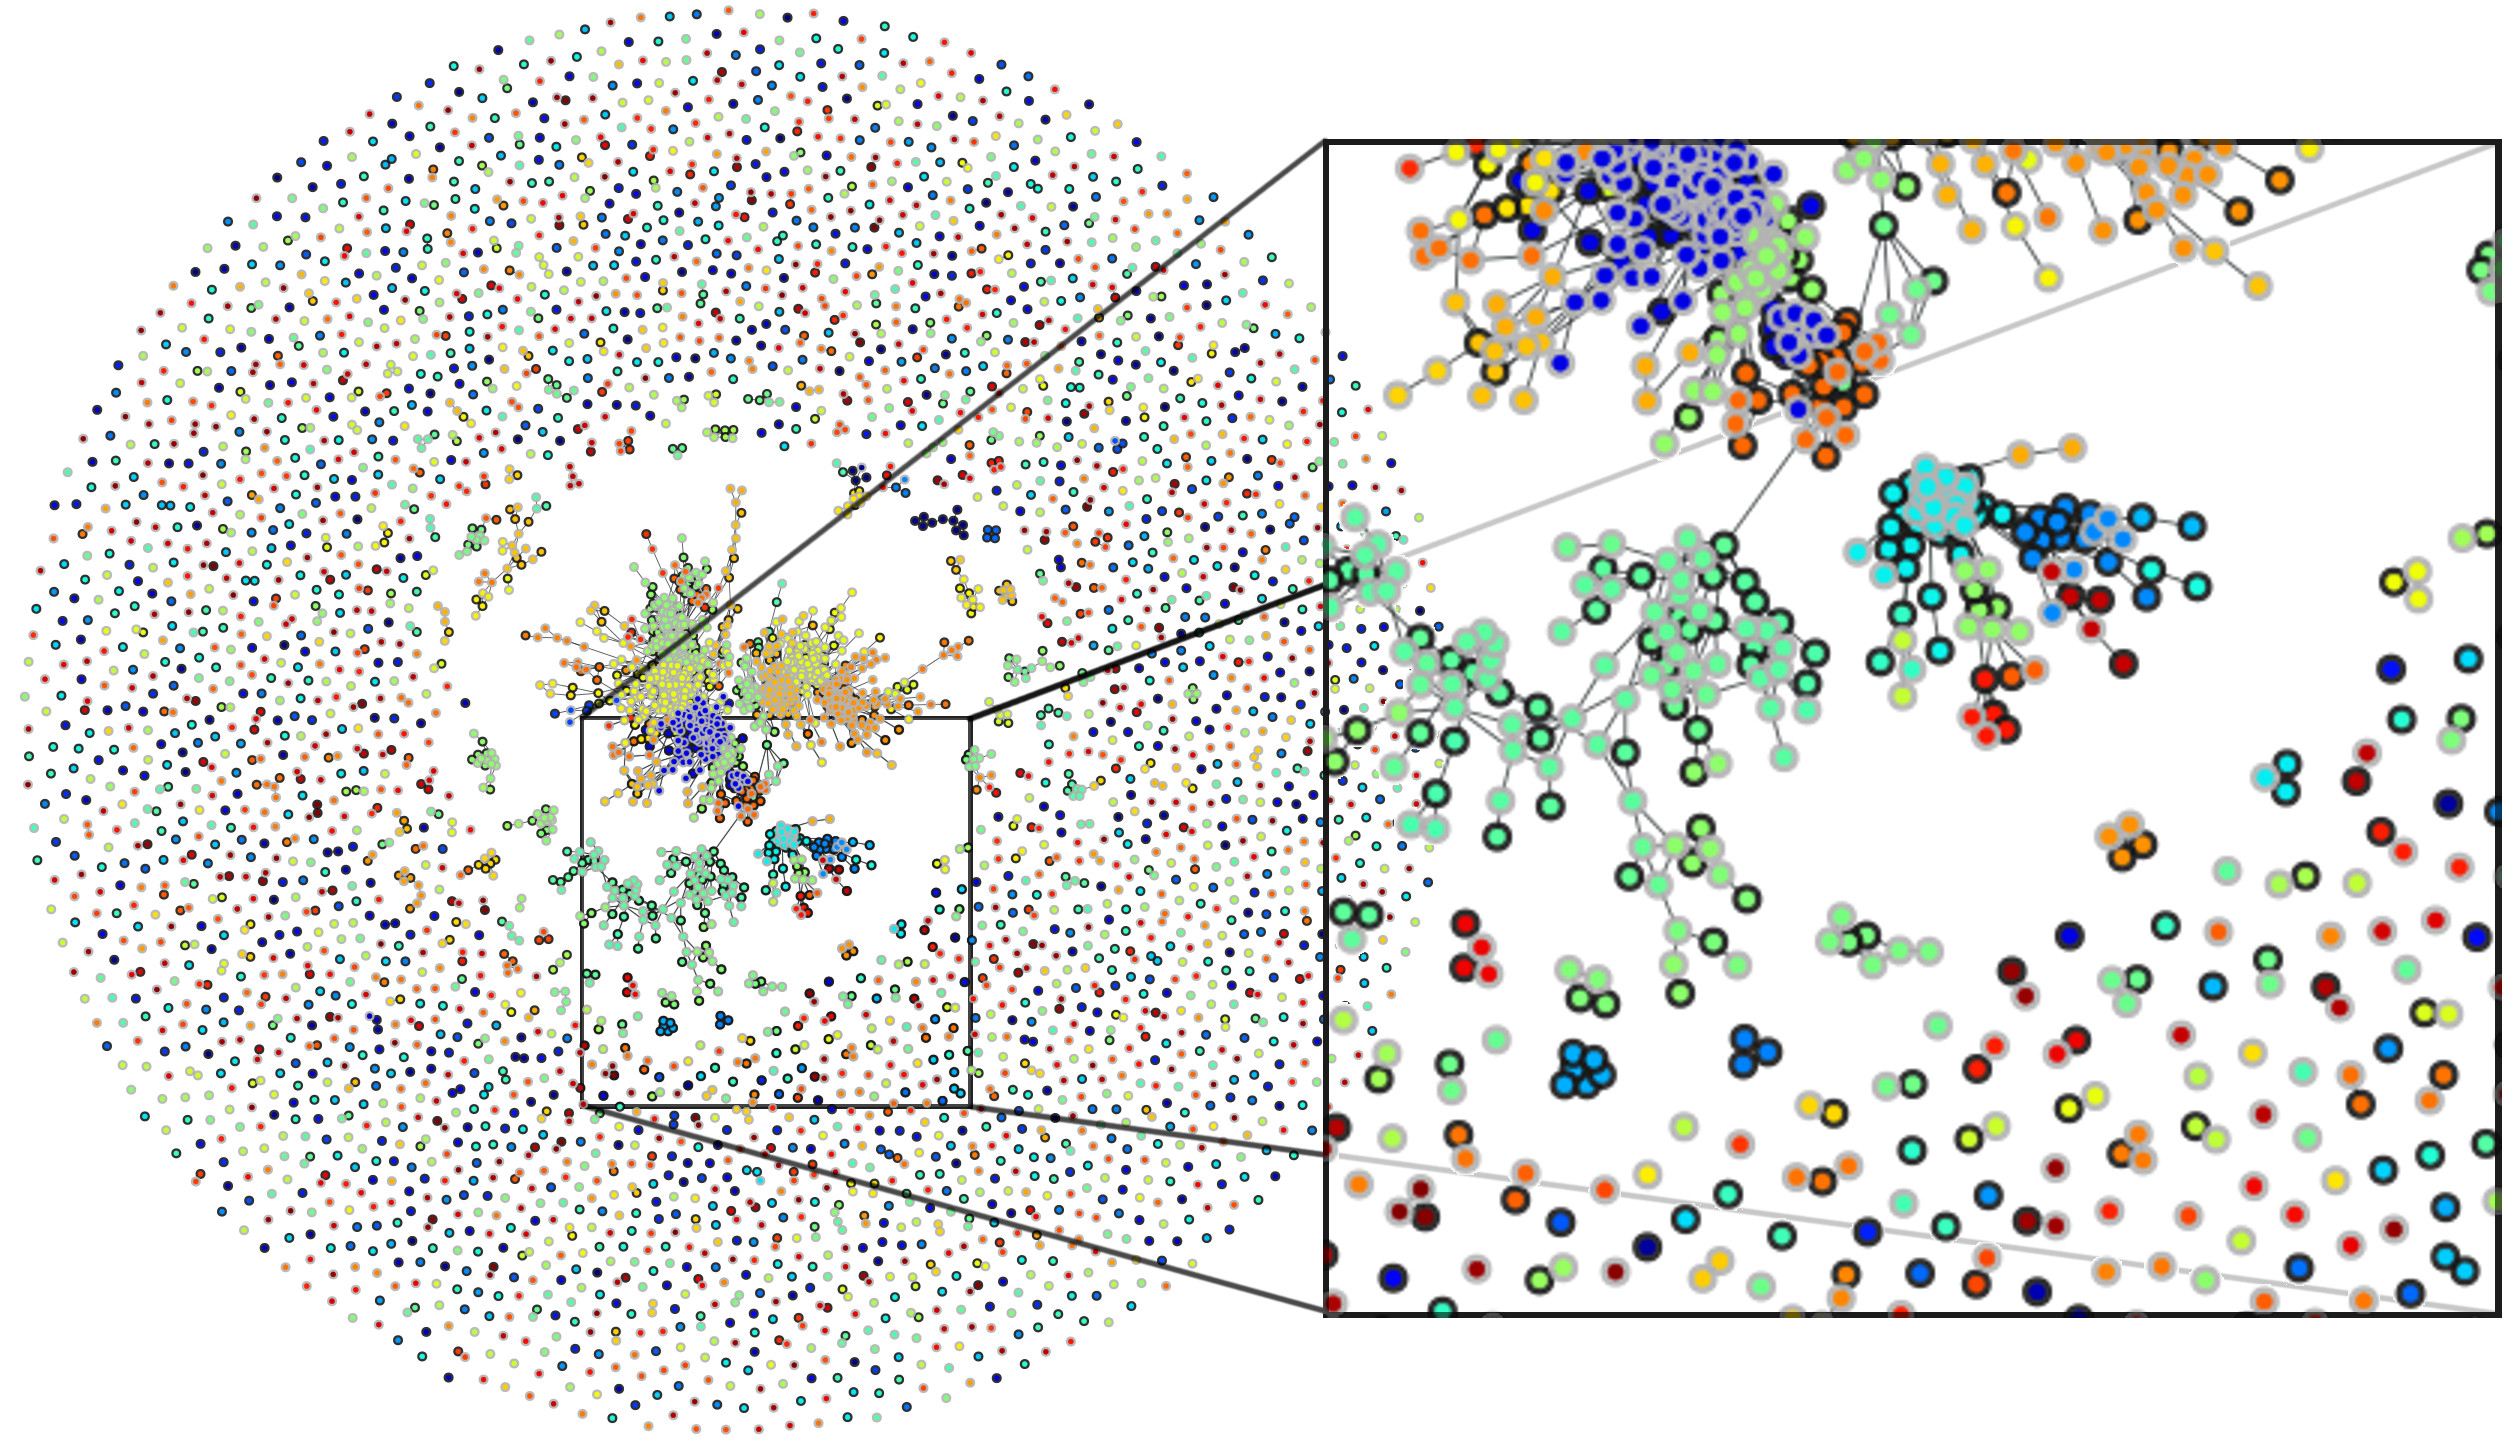
\includegraphics[width=1.1\textwidth]{images/MMC_graph}
    \label{fig:graph}
}
    \caption{The partitioned feature graph. Each vertex represents a 
        feature point; lines indicate high similarity between points. A 
        partition is a connected group with the same color. The border 
        color of each node indicates which image it belongs to.  Zooming 
    into a subsection of the graph (right part), the various cluster 
sizes can be seen, ranging from hundreds of feature points to only two 
or three.}
	\label{fig:graph}
\end{figure}

We use the Louvain Method \cite{blondel2008} for clustering feature 
points, since it is relatively fast and performs well 
\cite{lancichinetti2009}, does not require parameters 
\cite{blondel2008}, and does not emphasize partitions of equal size, as 
opposed to spectral clustering or k-means \cite{von2007}, for example.
While the Louvain clustering algorithm does not require any parameters 
in itself, it tends towards clustering all feature points together in 
the same partition if the graph is very connected.  To ensure that the 
graph is well clustered, the adjacency matrix is pruned so that only 
edges above a certain threshold are kept. From empirical analysis, 
retaining the top 2.5\% of edges with the highest similarity seems to 
work well in practice. Figure~\ref{fig:graph} shows the result of 
clustering the feature points as a graph.
%

The partitions group feature points by similarity, which means that 
repetitive structures such as buildings often appear in larger 
partitions, as exemplified in Figure~\ref{fig:pitts_partition}.
%

\begin{algorithm}
\caption{Impl.\ of getMatches (\emph{from MMC algorithm})}
\label{alg-getmatches}
    \fontsize{10}{10}\selectfont
    \begin{algorithmic}
    \Require $p$ : set of features, $t\in \mathbb{R}$, $features$ : Set of 
    all features
    \State $edges \gets \left\{similarity(f_i, f_j) \mid getImg(f_i)
        \neq getImg(f_j) \wedge f_i, f_j \in p \right\}$
    \If{$\left\vert edges \right\vert > 1$}
        \State $matches \gets MMGet(p, t)$
    \ElsIf{$\left\vert edges \right\vert = 1$}
        \State $matches \gets RatioGet(p, features, t)$
    \Else
        \State $matches \gets \varnothing$
    \EndIf

    \Return matches
    \end{algorithmic}
\end{algorithm}

The matching algorithm for \emph{MMC} detailed in 
Algorithm~\ref{alg-getmatches} finds matches within all partitions with 
more than two elements using the \emph{MM} approach.  However, as can be 
seen in the example in Figure~\ref{fig:MMC_graph}, many of the 
partitions contain only two feature points from different images linked 
by one edge. In this case, we compare the similarity of the these two 
feature points with their second best match and remove matches where 
this ratio lies above a certain threshold, like in the \emph{Ratio} 
algorithm.  For example in the case of Figure~\ref{fig:pitts_partition}, 
we have feature points from a building in one image grouped together 
with points from a shirt pattern in another.  The nearest neighbor 
method would have returned wrong matches, but since we match the 
partition with \emph{MM}, points in the building end up matching other 
points in the building, and no matches are returned.




\subsection{Experiments}
\label{S:Experiments}
%
To reliably measure the accuracy of a matching method on real images, we 
either need a set of image pairs tied by a homography, or we have to 
manually count the number of inliers. The latter becomes prohibitive for 
large numbers of (non-trivial) images. 

Mikolajczyk and Schmid  \cite{mikolajczyk2005performance} introduced a 
set of test images to compare the performance of feature detectors. The 
set covers different types of image variations, such as lighting change, 
blur, rotation, and viewpoint change. Inspired by this dataset (in 
particular the `Graf' image set) and motivated by the need for more 
image pairs featuring viewpoint changes, we have compiled a set of 8 
image pairs consisting of subjects taken from two different angles. The 
images are collected from Flickr's database of images published under a 
creative commons licence and feature murals, which makes it possible to 
relate points in the image pairs with a homography since most of the 
points in the images will be lying on a plane.  The images have been 
cropped to show the same motive and resized to $900\times 600$ pixels.  
This dataset will be referred to as the \emph{Murals} dataset.  
Figure~\ref{fig:murals} shows one image from each pair.

\begin{figure}[htb]
    \makebox[1.0\textwidth][c]{%
        \begin{subfigure}[t]{0.102\textwidth}
			\centering
			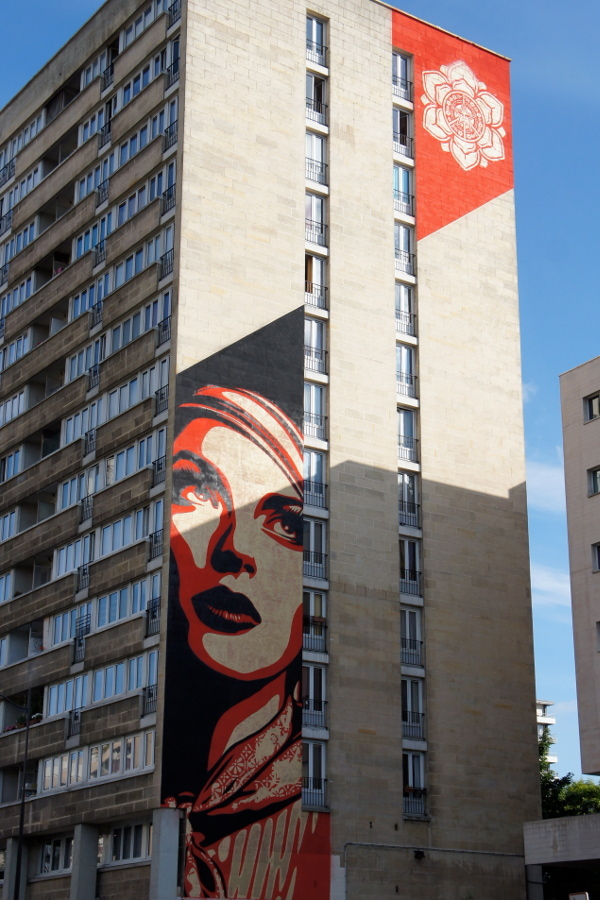
\includegraphics[width=\textwidth]{images/pair_example1}
			\label{fig:fairey1}
	\end{subfigure}%
		\enspace %add desired spacing between images, e. g. ~, \quad, 
		%(or a blank line to force the subfigure onto a new line)
        \begin{subfigure}[t]{0.102\textwidth}
			\centering
			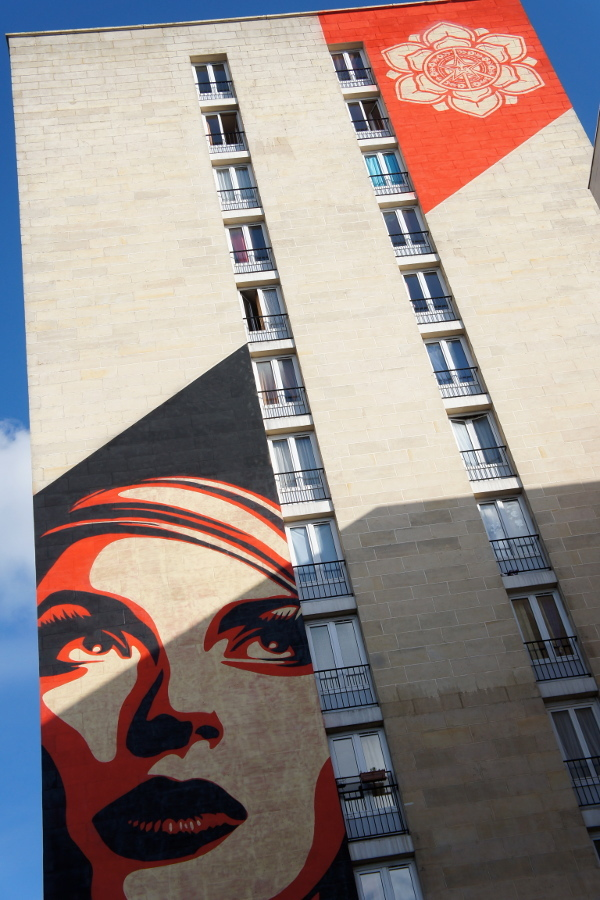
\includegraphics[width=\textwidth]{images/pair_example2}
			\label{fig:fairey2}
		\end{subfigure}%
		\enspace %
        \begin{subfigure}[t]{0.77\textwidth}
   		\centering
   		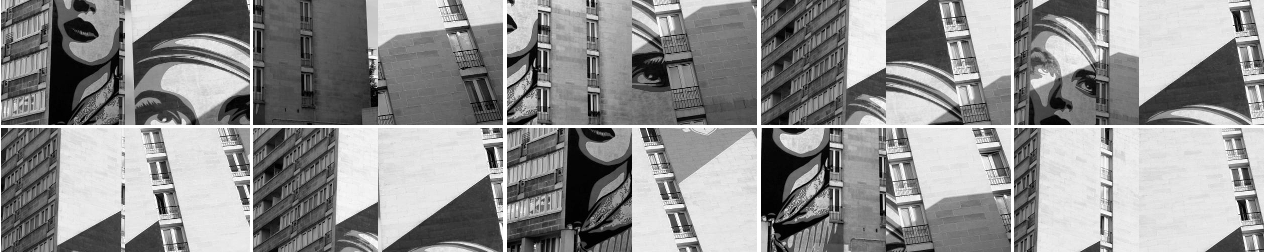
\includegraphics[width=\columnwidth]{images/crop_examples}
		\end{subfigure}%
	}%
	\caption{Sample test patches produced from an image pair.}
	\label{fig:fairey}
\end{figure}

\begin{figure*}[t]
	\centering
	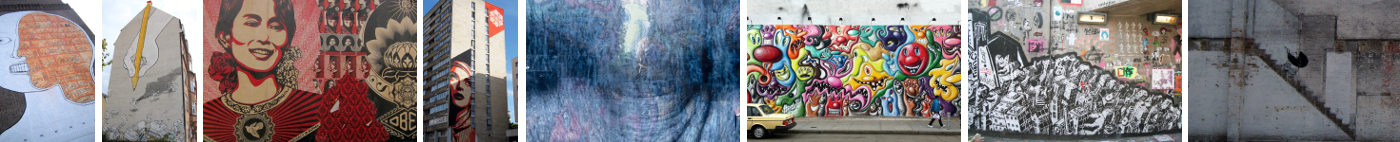
\includegraphics[width=\textwidth]{images/murals}
	\caption{Images in the \emph{Murals} test set.}
	\label{fig:murals}
\end{figure*}

\begin{figure}[htb]
	\centering
	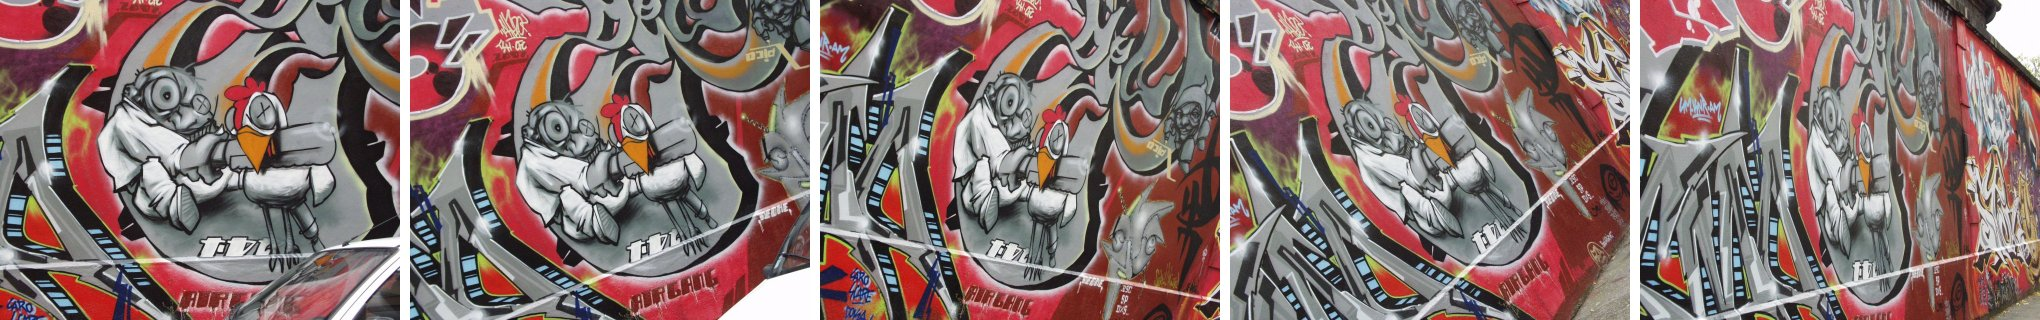
\includegraphics[width=\columnwidth]{images/graf12345.jpg}
	\caption{Images 1-5 of the Graf set from \cite{mikolajczyk2005performance}.}
	\label{fig:Graf}
\end{figure}


\subsubsection{Experimental setup}
We compare the \emph{MM} and \emph{MMC} algorithms to \emph{Ratio} 
\cite{lowe2004sift} as well as \emph{Isodata} \cite{das2008event} and 
\emph{Spectral} \cite{leordeanu2005spectral}.  \emph{Isodata} and 
\emph{Spectral} uses geometric constraints, whereas \emph{Ratio} does 
not.

\begin{algorithm}
\caption{Ratio Match (\emph{Ratio})}
\label{alg-ratio}
%{\fontsize{10}{10}\selectfont
\begin{algorithmic}
\Require $im_1$ : image, $im_2$ : image, $t \in \mathbb{R}$
\State $matches\gets \varnothing$
\State $features_1 \gets getFeatures(im_1)$
\State $features_2 \gets getFeatures(im_2)$
\ForAll{$f_i \in features_1$}
    \State $f_m,f_n \gets get2NNs(f_i, features_2)$
	\State $ratio \gets similarity(f_i, f_n) / similarity(f_i, f_m)$
	\If{$ratio < t$}
        \State $matches \gets \left(f_i, f_m\right)$
	\EndIf
\EndFor
\Return $matches$
\end{algorithmic}
%}
\end{algorithm}

\emph{Ratio} (Algorithm~\ref{alg-ratio}) \cite{lowe2004sift} is the most 
straightforward of the three reference algorithms. Feature points are 
matched using K Nearest Neighbor and the similarity ratio between the 
best and second best match is then compared to a threshold to decide if 
the match is kept.

\begin{algorithm}
\caption{Isodata Match (\emph{Isodata})}
\label{alg-isodata}
%{\fontsize{10}{10}\selectfont
\begin{algorithmic}
\Require $im_1$ : image, $im_2$ : image, $t \in \mathbb{R}$
\State $matches_{init}\gets \varnothing$
\State $matches_{final}\gets \varnothing$
\State $features_1 \gets getFeatures(im_1)$
\State $features_2 \gets getFeatures(im_2)$
\ForAll{$f_i \in features_1$}
    \State $f_m,f_n \gets get2NNs(f_i, features_2)$
    \State $matches_{init} \gets \left(f_i, f_m\right)$
\EndFor
\State $partitions_1 \gets isodata(getPositions(features_1))$
\State $partitions_2 \gets isodata(getPositions(features_2))$
\State $P_{corr} \gets getMatchMat(partitions_1, partitions_2, 
matches_{init})$
\ForAll{$(i,j) \in indices(P)$}
    \If{$\left(P_{i,j} > 5\right) \wedge \left(P_{i,j} / sum(P_{i}) > 
    0.5\right)$}
        \State $matches_{final} \gets getMatches(matches_{init}, 
        partitions_1, partitions_2, i, j)$
    \EndIf
\EndFor
\Return $matches_{final}$
\end{algorithmic}
%}
\end{algorithm}

The \emph{Isodata} algorithm (Algorithm~\ref{alg-isodata}) 
\cite{das2008event} is based on the idea that local feature points 
within a region in one image often matches to features within a 
corresponding region in the other image. To find these regions the 
algorithm uses the Isodata algorithm \cite{ball1965isodata} to perform 
unsupervised clustering on the feature points given their positions in 
the two images. The Isodata algorithm is similar to K-means with the 
addition that clusters are merged and split during the clustering 
process. The initial set of matches are then filtered based on the 
resulting regions. A match is kept only if it belongs to a region with 
more than 5 matches and where half of the matches link the same two 
regions. $P_{corr}$ in Algorithm~\ref{alg-isodata} is a matrix where 
each row corresponds to a region in $im_1$, each column corresponds to a 
region in $im_2$ and $P_{i,j}$ is the amount of matches going from 
region $i$ to region $j$.

There is no inherent threshold parameter in \emph{Isodata} so to show 
how the algorithm performs over.
%, which uses geometric information to improve the matching.  The 
%comparison  with \emph{Ratio} serves to illustrate the relative 
%performance of \emph{MM} and \emph{MMC} to a state of the art algorithm 
%without geometric constraints. \emph{Isodata} is included to illustrate 
%the performance of an algorithm relying on geometric constraints faced 
%with image pairs that might not have any overlap.  
The comparison was done using the \emph{Murals} dataset 
(Figure~\ref{fig:murals}), the \emph{Graf} set (Figure~\ref{fig:Graf}) 
from \cite{mikolajczyk2005performance}, and two 
images\footnote{100\_1942.jpg and 100\_1941.jpg} from the Gallagher 
dataset \cite{gallagher2008} (Figure~\ref{fig:comparemirror}).

Test sets were generated from the image pairs by cropping square patches of
$250\!\times\!250$ pixels with a random vertical and horizontal offset.  
Given a source image pair, we produce 100 pairs of patches, which might or might not overlap.  
This ensures that patch pairs with no overlap still retain a general similarity to each 
other, while patches that do overlap often only share a small 
part of their area. Figure~\ref{fig:fairey} shows an example of 
possible pairs of test image patches produced from a source image pair.  
Producing $n$ such pairs allows us to test not just how well the 
matching algorithm performs on a variety of overlaps but also how many 
false positives we get on similar images that do not overlap at all. In 
practice the amount of overlap between pairs in a test set will depend 
on the overlap and viewpoint change in the source image pair.  To give a 
rough idea, Table~\ref{table:overlap} shows the overlap of patch pairs 
created from images 1 and 3 of the \emph{Graf} image set from 
\cite{mikolajczyk2005performance}.

\begin{table}[htb]
\caption{Overlap in the set of 100 patch pairs created from two images 
of the \emph{Graf} image set (Figure~\ref{fig:Graf}).}
\label{table:overlap}
    \centering
%   \small
\begin{tabular}{r*{3}{r}}
\hline
    Amount of overlap: & 0\% & $< 50$\% & $> 50$\%  \\
    \noalign{\smallskip}
	%
    Number of patch pairs: & 21 & 54 & 25 \\
    \hline
\end{tabular}
\end{table}

Given a potential match between two pixels $p_1$ and $p_2$, $m = 
\left(p_1, p_2\right)$, and a homography $H$ relating the two images 
$I_1$ and $I_2$, we can calculate if $m$ is an inlier by checking if the 
two points satisfy the following criteria:
\begin{equation*}
\left\vert H p_1 - p_2 \right\vert + \left\vert H^{-1}p_2 - p_1 \right\vert < d_{\max}
\end{equation*}
That is, the distance between $p_1$ translated to $I_2$ and $p_2$ 
\emph{plus} the distance between $p_2$ translated to $I_1$ should be 
less than a certain threshold (we use $d_{\max}=5$ pixels here).


\subsection{Results}
\label{S:Results}

Figure~\ref{fig:result_graf} shows the results for 100 patch pairs 
generated from images 1 and 3 of the \emph{Graf} image set 
(cf.~Figure~\ref{fig:Graf}). The plot compares the accuracy of 
\emph{Ratio}, \emph{MM}, \emph{MMC}, and \emph{Isodata} as a function of 
the number of matches produced (which is achieved by varying thresholds 
over a certain range). The results show that \emph{MM} and \emph{MMC} 
consistently outperform \emph{Ratio}; \emph{MMC} generally lies 2-3 
percentage points above \emph{MM} when both are performing at optimal 
accuracy.  Although \emph{Isodata} exhibits a good performance on strict 
thresholds (small number of matches), that quickly diminishes when more 
matches are desired.


\begin{figure}[htb]
%	\makebox[0.5\textwidth][c]{%
%		\begin{subfigure}[t]{.13\textwidth}
%			\centering
%			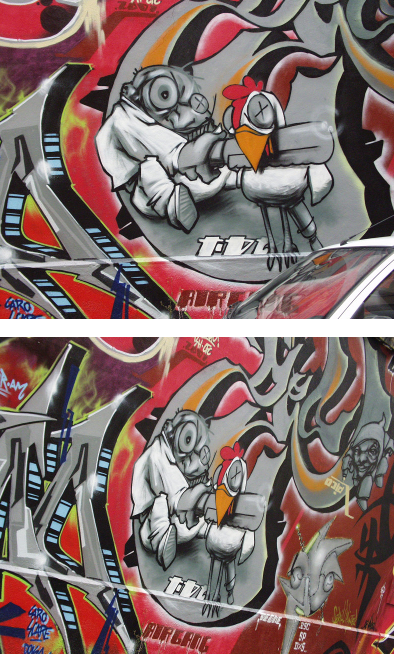
\includegraphics[width=\textwidth]{images/graf}
%		\end{subfigure}%
%		~ %add desired spacing between images, e. g. ~, \quad, \qquad		  
		%(or a blank line to force the subfigure onto a new line)
%		\begin{subfigure}[t]{.27\textwidth}
			\centering
			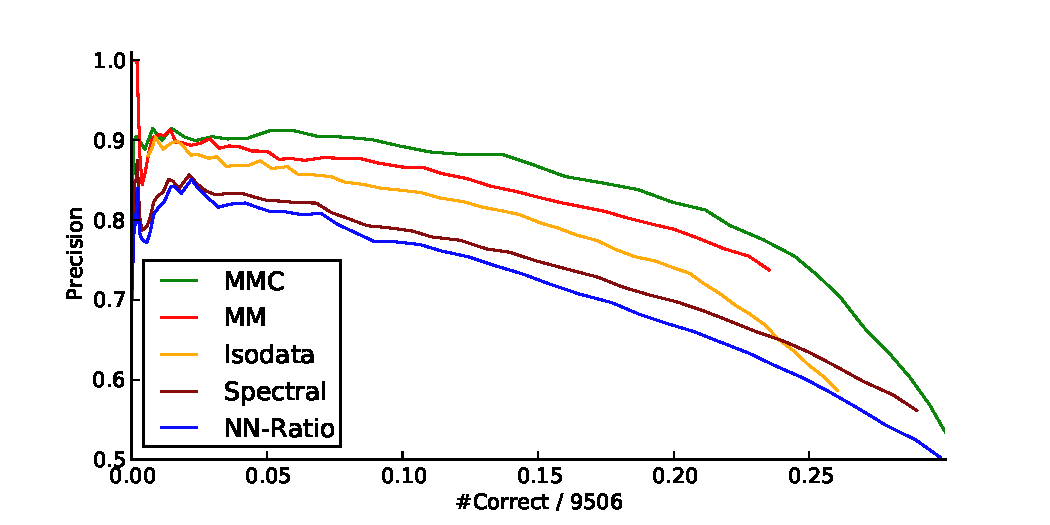
\includegraphics[width=0.6\columnwidth]{images/result_graf}
			%\caption{Performance on Scharf}
%		\end{subfigure}%
%	}%
	\caption{Accuracy for image pair 1\&3 from the \emph{Graf} set. The plot 
		shows the result of 100 patch pairs generated from the source 
		images shown to the left. The number of matches is the total 
		number of matches for all 100 patch pairs.}
	\label{fig:result_graf}
\end{figure}

To validate whether these results 
generalize to other images, we tested the four algorithms on the 
\emph{Murals} dataset as well as the \emph{Graf} pair tested above.  
In total 900 different patch pairs were generated from 9 
source image pairs.  The results are shown in Figure 
\ref{fig:result_accumulated}. 

\begin{figure}[htb]
	\centering
	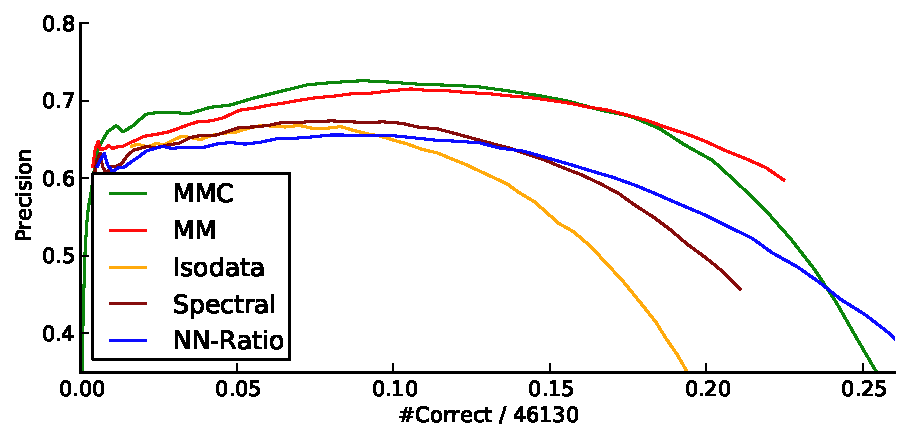
\includegraphics[width=\columnwidth]{images/result_accumulated}
	\caption{Results for 900 patch pairs extracted from the \emph{Murals} dataset and the image pair 1\&3 from the \emph{Graf} set.  The x-axis shows the accumulated returned matches for all pairs.}
	\label{fig:result_accumulated}
\end{figure}

To further investigate the impact of viewpoint changes, we tested the 
algorithms on the \emph{Graf} image set (Figure~\ref{fig:Graf}), which 
contains 5 images of the same mural taken with gradually increasing 
viewpoint changes.  The first images are almost identical, while the 
last are taken from very different angles. The results from   \emph{MMC} 
and \emph{Ratio} as shown in Figure~\ref{fig:result_viewpoint}, 
confirming that \emph{MMC} is generally superior to \emph{Ratio} across 
viewpoint changes.
The performance of \emph{MM} (not shown in the plot) is similar to 
\emph{MMC}.

\begin{figure}[htb]
	\centering
	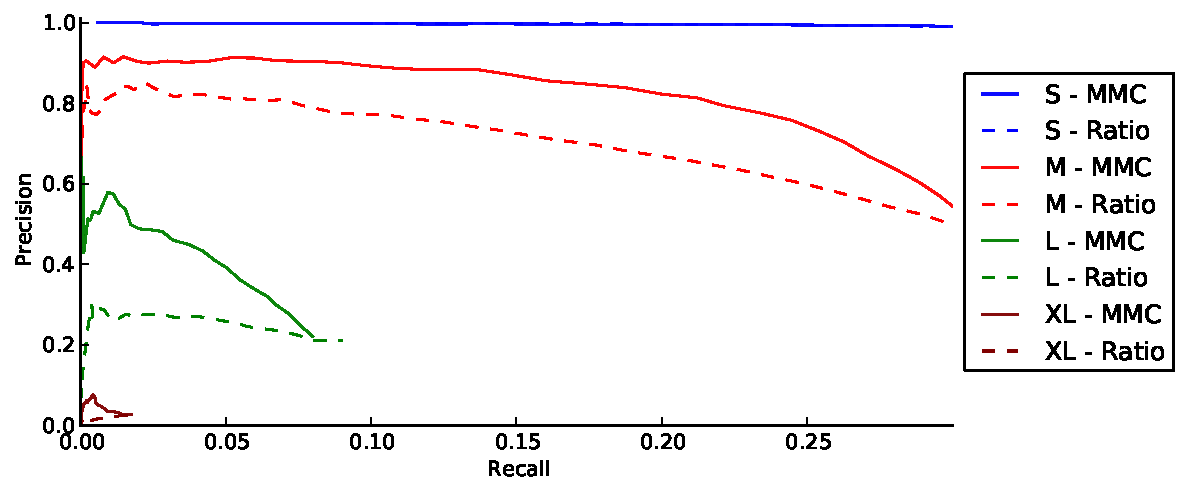
\includegraphics[width=0.45\textwidth]{images/result_viewpoint}
	\caption{Results for viewpoint changes using the \emph{Graf} set from 
		\cite{mikolajczyk2005performance}.  S: img1\&2; M: img1\&3; L: img1\&4; XL: img1\&5.}
	\label{fig:result_viewpoint}
\end{figure}


Finally, for an example of a real life use case, Figure~\ref{fig:result_pitts} 
shows the results on 100 patch pairs generated 
from a typical holiday photo shot (Figure~\ref{fig:pitts_source}) featuring occlusion and a slight viewpoint 
change from the Gallagher dataset \cite{gallagher2008}.  The performance is comparable to the murals, despite the lack of a simple homographic mapping between the images.


\begin{figure}[htb]
%	\makebox[0.5\textwidth][c]{%
%		\begin{subfigure}[t]{.15\textwidth}
%			\centering
%			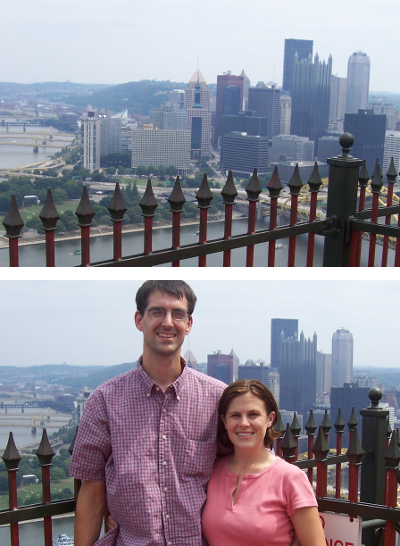
\includegraphics[width=\textwidth]{images/pitts}
%		\end{subfigure}%
		~%add desired spacing between images, e. g. ~, \quad, \qquad
		%(or a blank line to force the subfigure onto a new line)
%		\begin{subfigure}[t]{.27\textwidth}
			\centering
			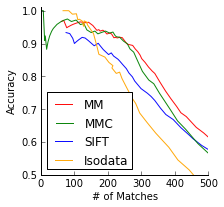
\includegraphics[width=0.6\columnwidth]{images/result_pitts}
			%\caption{Performance on Scharf}
%		\end{subfigure}%
%	}%
	\caption{Results for the image pair in Figure~\ref{fig:pitts_source}.}
	\label{fig:result_pitts}
\end{figure}


In terms of computational complexity, \emph{Ratio}, \emph{MM}, and \emph{Isodata} can be 
implemented in $O(n\log n)$, where $n$ is the total number of feature 
points.  Our current \emph{MMC} implementation has a complexity of $O(n^2)$ due to the 
construction of a similarity matrix of the feature points. However, it is 
possible to approximate this in $O(n\log n)$ using search trees.  

As for speed, Table~\ref{table:running_times} shows the running time of 
the four algorithms over 100 image pairs of $250\!\times\!250$ pixels.  
These numbers should be taken with a grain of salt, given that much of 
the code behind \emph{MMC} and \emph{Isodata} is implemented in Python, 
whereas \emph{MM} and \emph{Ratio} make use of OpenCV to execute 
computationally intensive operations in C++, which makes them much 
faster. 

\begin{table}[htb]
\caption{Running times as tested on a Intel\textregistered\ Core\texttrademark\ i5-3550 CPU @ 
3.30~GHz with 8~GB memory.}
\label{table:running_times}
	\centering
%	\small
\begin{tabular}{r*{4}{c}}
\hline
	Algorithm: & \emph{Ratio} & \emph{MM} & \emph{MMC} & \emph{Isodata} 
	\\
	\noalign{\smallskip} 
	%
	Running time: & 20.94s & 18.23s & 883.99s & 555.33s \\
	\hline
\end{tabular}
\end{table}
%

\section{Applications}

In many areas of computer vision matching local feature points is a key 
component, and matching algorithms have applications in problems such as
scene matching, object recognition, near duplicate detection and 
panorama recognition. To show the practical applications of the proposed 
matching algorithms, \emph{MM} and \emph{MMC}, we use show how they 
improve existing methods in near duplicate detection and panorama 
recognition. These two problems were chosen because they both involve 
matching images that might or might not overlap. These cases requires 
matching algorithms that limit false positives since e.g. returning the 
top $n$ matches for any given image pair would make it hard to 
distinguish adjacent or duplicate images from non-adjacent or dissimilar
image pairs. Near duplicate detection also constraints normal matching 
algorithms from relying on geometric assumptions, since we have very few
guarantees between two potential near duplicates that they should be 
matched using any particular geometric heuristic. In this section, we 
will first see \emph{MMC} applied to panorama recognition and alignment,
and next \emph{MM} and \emph{MMC} applied to near duplicate detection.


\subsection{Panorama Recognition and Alignment}
One of the oldest practical problems approached in computer vision is 
the automatic stitching of several source images into a bigger image, 
such as panoramas and composite satellite photos\footnote{A brief 
overview of the history of image stitching can be found in Szeliski's 
book: Computer Vision: Algorithms and Applications \cite{szeliski2010}}.  
As part of the process of stitching together images, the individual 
images must be aligned and often transformed in perspective. Earlier 
methods relied on minimizing pixel dissimilarities in overlapping images 
while more recent methods have used local feature points to estimate the 
correct image alignment. Using local feature points carry the additional 
advantage that it is feasible to automatically recognize where each 
source image belong in the final panorama.

\begin{figure}[h]
	\begin{subfigure}[t]{0.9\textwidth}
		\centering
        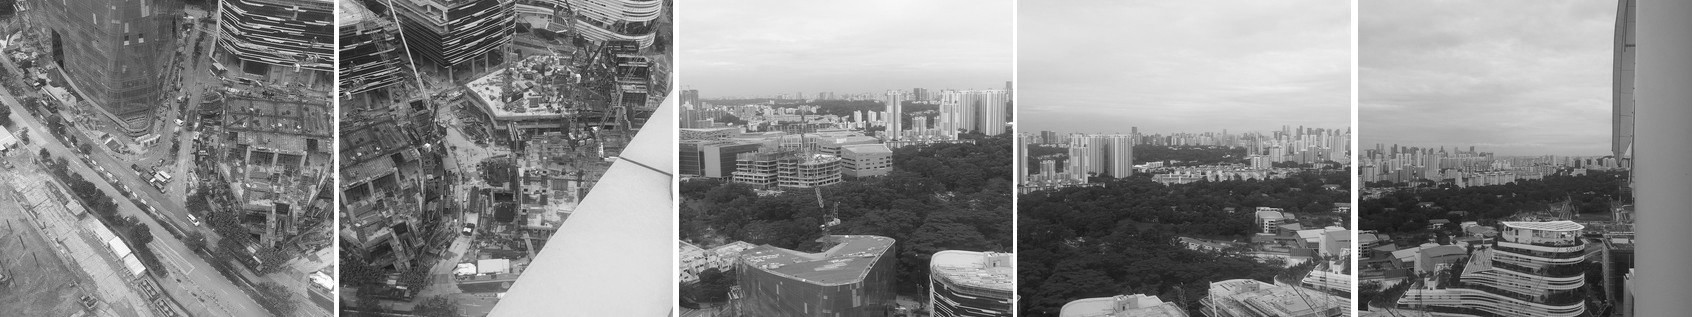
\includegraphics[width=\textwidth]{images/pano_wide}
        \label{fig:pano_images}
		\caption{Source images}
    \end{subfigure}%
	\\
	\centering
    \begin{subfigure}[b]{0.4\textwidth}
		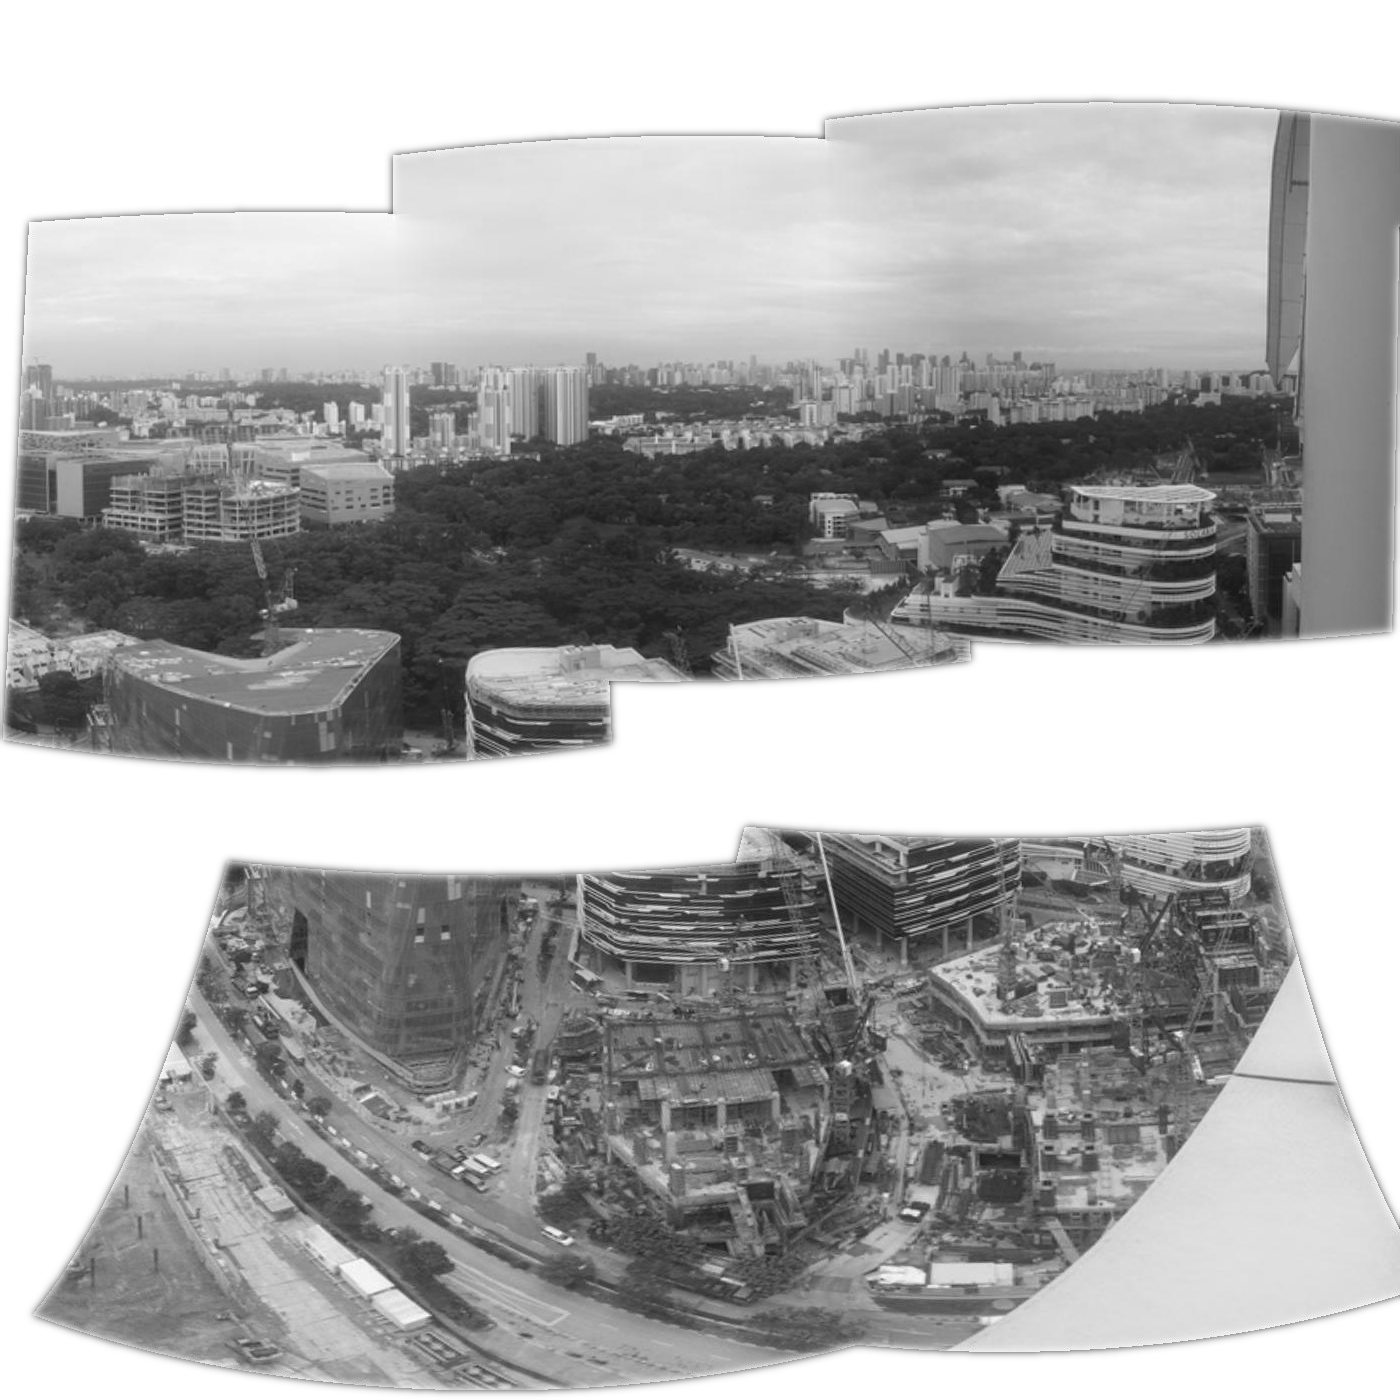
\includegraphics[width=\textwidth]{images/panorama-autostitch}
        \label{fig:pano_autostitch}
		\caption{Panorama by Autostitch}
    \end{subfigure}%
	~%add desired spacing between images, e. g. ~, \quad, \qquad
	%(or a blank line to force the subfigure onto a new line)
    \begin{subfigure}[b]{0.4\textwidth}
		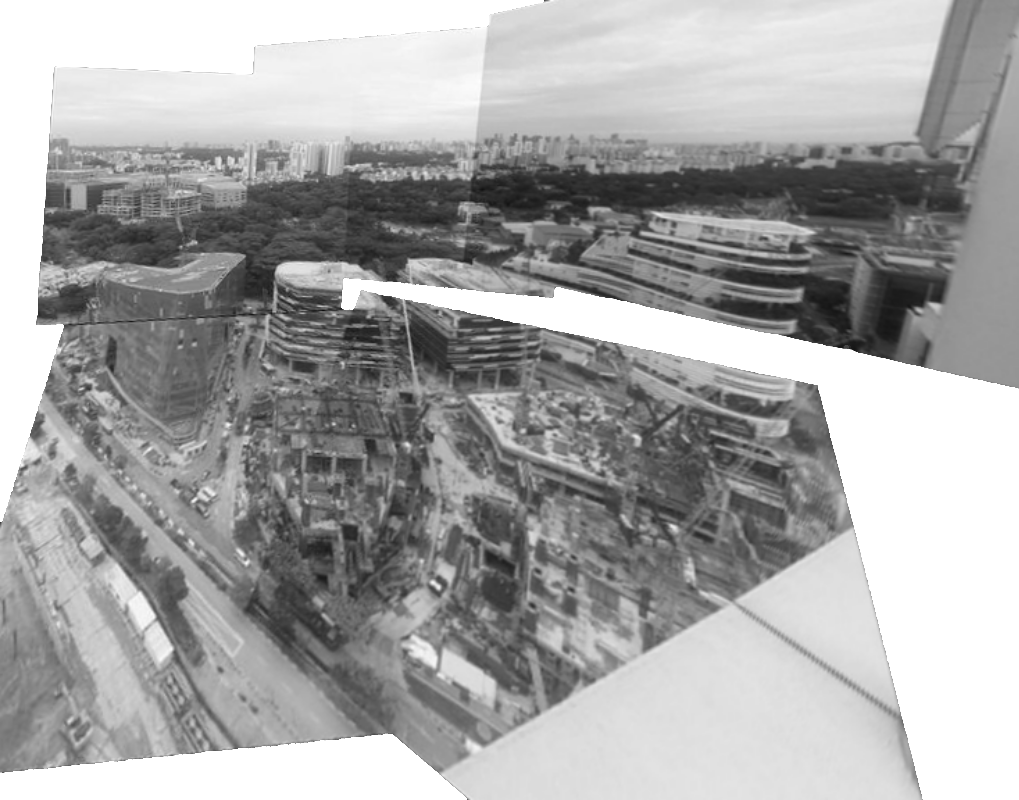
\includegraphics[width=\textwidth]{images/panorama-MMC}
		\caption{Panorama by MMC}
		\label{fig:pano_MMC}
	\end{subfigure}%
    \label{fig:pano_example}
	\caption{An example of a difficult case for panorama recognition and 
		alignment.  In a) the source images used to generate the 
		panorama are displayed.\ b) shows the result of the Autostitch 
		program from \cite{brown2007automatic} which fails to combine 
		all images, while c) demonstrates the result of the simple 
		panorama stitcher
	using the proposed MMC algorithm. Here the two left images are 
correctly linked}
\end{figure}

In \cite{brown2007automatic}, Brown and Lowe demonstrate how a panoramic 
image can be assembled by collecting the feature points of all source 
images and matching them to obtain a set of inter image matches.  By 
using \emph{RANSAC}\footnote{RANdom SAmple Consensus, an iterative 
    algorithm to estimate parameters from noisy data introduced in 
Fischler and Bolles in 1981 \cite{fischler1981ransac}} to find matches 
deemed as inliers between image pairs, they are able to recognize image 
neighbors and align them to construct the final panorama.

This process hinges on the effectiveness of the matching algorithm used 
to match the feature points. Not only is it important that true pairs 
are accurately matched, but since we are matching points in image pairs 
that might not be adjacent in the final panorama, we also need to make 
sure that we consistently reject false positives, i.e.\ proposed matches 
that link feature points which don't correspond.

To demonstrate the usefulness of \emph{MMC} applied to panorama 
recognition and alignment we construct a simple panorama stitcher taking
as input a set of $n$ source images $\left\{I_0, \ldots, I_n\right\}$ 
and returns as output a panoramic image stitched together from the 
source images. Based on the matches found by applying \emph{MMC} to $I$, 
the images are combined in an order corresponding to how many matches 
connect them, as done by Brown and Lowe \cite{brown2007automatic}.

Brown and Lowe make use of bundle adjustment\footnote{Bundle adjustment 
provides a way to globally optimize the accuracy of the image alignment} 
and a lot of image enhancements such as exposure adjustment and edge 
blurring to provide a seamless panorama. While these additions improve 
the end product, they don't influence the performance of panorama 
alignment and recognition and haven't been included in the simple 
comparison algorithm.

Figure~\ref{fig:pano_example} shows an example where the added accuracy 
of MMC enables us to correctly recognitize and align source images that 
fail to be combined by Autostitch, a program using the algorithm 
proposed by Brown and Lowe \cite{brown2007automatic}. In this particular
case the matching algorithm used in Autostitch fails to find sufficient 
matches between two images pairs to correctly position them and 
consequently doesn't produce a panorama containing all images as a 
result.

This example illustrates how an improved matching algorithm can be 
applied to panorama recognition and alignment to allow for panoramas 
created with images that have little overlap.
% Maybe find example of images with identical features that would be 
% hard to match?

\subsection{Near Duplicate Detection}
If we look at two images, we can often easily tell if one image 
resembles the other enough to be redundant in a photo album. In computer 
vision this task becomes a lot less trivial because our idea of a 
duplicate image might only require there being some object or scene in 
common between the image pair. In addition the object or scene might 
have been taken from a different angle and under different camera 
settings. Facing these challenges, a lot of work has been done trying to 
reliably recognize duplicaes both with regards to corporate intellectual 
property as well as consumer photo albums because both applications 
provide useful tools.  A company might be interested in finding images 
that are derived from their intellectual property, while consumers 
taking vacation photos might be interested in grouping duplicate images 
to allow for easier photo organization.

Local features are often used to group similar images, either by looking
at a histogram of descriptors \cite{wu2009bundling} or by looking at how
well feature points match between images \cite{zhao2009scale},
\cite{chu2010consumer}, \cite{vas2013cluster}. In the latter case 
finding near duplicates means that we will be matching image pairs that 
might or might not contain any actual matches. In this case we would 
benefit from a reliable matching algorithm that minimizes false 
positives, which is a characteristic of both \emph{MM} and \emph{MMC}.

The \emph{PhotoCluster} method introduced by Vonikakis et al.  
\cite{vas2013cluster} shows the best clustering performance on the 
California-nd dataset \cite{jinda2012california} which contains a set of
annotated vacation images similar to a typical photo album in a consumer
product. \emph{PhotoCluster} works by grouping images in several steps 
using first image metadata and global features to obtain a set of 
proposed clusters. Then local features are used to find the best 
matching images in these proposed clusters yielding the final groups of 
near duplicate images. To show the viability of \emph{MMC} in the 
application of near duplicated detection, we modify the PhotoCluster 
method to use \emph{MMC} for matching images instead of \emph{Ratio} 
which was previously used. Due to the time consumption of \emph{MMC}, 
all images where resized to to 10\% before being compared. Outside of 
that, the experiments were performed exactly as documented in 
\cite{vas2013cluster}.

\begin{table}[htb]
\caption{Results from Near Duplicate Detection at 10\% scale}
\label{table:ndd}
	\centering
%	\small
\begin{tabular}{r*{2}{r}}
\hline
    Method: & Ratio & MMC   \\
	\noalign{\smallskip}
	%
    F1 score: & 0.4654 & 0.5459 \\
	\hline
\end{tabular}
\end{table}

The results of the comparison can be seen in Table~\ref{table:nnd}. It 
shows that \emph{MMC} improves performance by 8.05\% over the original 
framework using \emph{Ratio} to match images. For comparison, the 
performance improvement of \emph{PhotoCluster} compared to XMatch 
\cite{zhao2009scale}, the second best performing algorithm on the 
California-nd dataset according to \cite{vas2013cluster}, is 2.52\%.

\section{Summary}
\label{S:Summary}

This thesis has addressed the problem of matching feature points without 
using geometrical constraints, proposing \emph{Mirror Match (MM)} and 
\emph{Mirror Match with Clustering (MMC)}.  The two algorithms share the 
common idea that feature points should have better matches in another 
image than in the image they came from to be considered good matches.  
\emph{MMC} further improves on this idea by using the structure of the 
similarity graph of the feature points. 

The algorithms show promising results when tested on the \emph{Murals} 
data set. The results on 900 image pairs show that \emph{MM} and 
\emph{MMC} generally outperform existing matching algorithms 
\emph{Ratio}, \emph{Isodata} and \emph{Spectral}. In addition \emph{MMC} 
outperforms \emph{MM}.  We show that this result generalizes to 
variations in viewpoint change by comparing \emph{MMC} to \emph{Ratio} 
over a set of image pairs with an increasing magnitude of perspective 
difference. We go on to apply the algorithms to a real life image case 
featuring occlusion and a slight viewpoint change and show that the 
performance of \emph{MM} and \emph{MMC} is consistent with the results 
on \emph{Murals}. To show that \emph{MM} or \emph{MMC}
can further improve the results of a geometrical method, we create 
\emph{Spectral-MMC} by combining \emph{Spectral} and \emph{MMC} and 
compare the three on the full \emph{Murals} dataset where it yields 
results better than both \emph{Spectral} and \emph{MMC}.

The practical application of \emph{MM} and \emph{MMC} is demonstrated by 
applying the algorithms to the problems of near duplicate detection and 
for the case of \emph{MMC} to panorama recognition and alignment. For 
the case of near duplicate detection, \emph{MMC} provides an 8.02\% 
improvement over \emph{Ratio} in a near duplicate detection framework 
making use of local features. Similarly for panorama recognition and 
alignment a simple panorama stitching method based on \emph{MMC} 
succeeds in cases where \emph{Autostitch} is unable to recognize and 
align the source images correctly. Both applications illustrate the 
central role that performance of the matching algorithm has on tasks 
that makes use of local features to match image pairs with potential 
overlap.
%

\bibliographystyle{IEEEtran}
\bibliography{bibliography}
\end{document}
